\documentclass{article}

\usepackage{fancyhdr}
\usepackage{extramarks}
\usepackage{amsmath}
\usepackage{amsthm}
\usepackage{amsfonts}
\usepackage{tikz}
\usepackage[plain]{algorithm}
\usepackage{algpseudocode}
\usepackage{enumerate}
\usepackage{tikz,forest}
\usepackage{multicol}
\usepackage{enumitem}
\usepackage{adjustbox}
\usepackage{bm}
\usepackage{listings}
\lstset{language=Matlab}   
%\usepackage[demo]{graphicx}

\newcommand{\norm}[1]{\left\lVert#1\right\rVert}

%
% Basic Document Settings
%

\topmargin=-0.45in
\evensidemargin=0in
\oddsidemargin=0in
\textwidth=6.5in
\textheight=9.0in
\headsep=0.25in

\linespread{1.1}

\pagestyle{fancy}
\lhead{\hmwkAuthorName}
\chead{\hmwkClass : \hmwkTitle}
\rhead{\firstxmark}
\lfoot{\lastxmark}
\cfoot{\thepage}

\renewcommand\headrulewidth{0.4pt}
\renewcommand\footrulewidth{0.4pt}

\setlength\parindent{0pt}

%
% Create Problem Sections
%

\newcommand{\enterProblemHeader}[1]{
\nobreak\extramarks{}{Problem \arabic{#1} continued on next page\ldots}\nobreak{}
\nobreak\extramarks{Problem \arabic{#1} (continued)}{Problem \arabic{#1} continued on next page\ldots}\nobreak{}
}

\newcommand{\exitProblemHeader}[1]{
\nobreak\extramarks{Problem \arabic{#1} (continued)}{Problem \arabic{#1} continued on next page\ldots}\nobreak{}
\stepcounter{#1}
\nobreak\extramarks{Problem \arabic{#1}}{}\nobreak{}
}

\setcounter{secnumdepth}{0}
\newcounter{partCounter}
\newcounter{homeworkProblemCounter}
\setcounter{homeworkProblemCounter}{1}
\nobreak\extramarks{Problem \arabic{homeworkProblemCounter}}{}\nobreak{}

%
% Homework Problem Environment
%
% This environment takes an optional argument. When given, it will adjust the
% problem counter. This is useful for when the problems given for your
% assignment aren't sequential. See the last 3 problems of this template for an
% example.
%
\newenvironment{homeworkProblem}[1][-1]{
\ifnum#1>0
\setcounter{homeworkProblemCounter}{#1}
\fi
\section{Problem \arabic{homeworkProblemCounter}}
\setcounter{partCounter}{1}
\enterProblemHeader{homeworkProblemCounter}
}{
\exitProblemHeader{homeworkProblemCounter}
}

%
% Homework Details
%   - Title
%   - Due date
%   - Class
%   - Section/Time
%   - Instructor
%   - Author
%

\newcommand{\hmwkTitle}{Problem Set\ \#6}
\newcommand{\hmwkDueDate}{November 10, 2017}
\newcommand{\hmwkClass}{CIS 520}
%\newcommand{\hmwkClassTime}{Section A}
\newcommand{\hmwkClassInstructor}{Lyle Ungar, Shivani Agarwal}
\newcommand{\hmwkAuthorName}{Eric Oh}

%
% Title Page
%

\title{
\vspace{2in}
\textmd{\textbf{\hmwkClass:\ \hmwkTitle}}\\
\normalsize\vspace{0.1in}\small{Due\ on\ \hmwkDueDate\ }\\
\vspace{0.1in}\large{\textit{\hmwkClassInstructor}}
\vspace{3in}
}

\author{\textbf{\hmwkAuthorName}}
\date{}

\renewcommand{\part}[1]{\textbf{\large Part \Alph{partCounter}}\stepcounter{partCounter}\\}

%
% Various Helper Commands
%

% Useful for algorithms
\newcommand{\alg}[1]{\textsc{\bfseries \footnotesize #1}}

% For derivatives
\newcommand{\deriv}[1]{\frac{\mathrm{d}}{\mathrm{d}x} (#1)}

% For partial derivatives
\newcommand{\pderiv}[2]{\frac{\partial}{\partial #1} (#2)}

% Integral dx
\newcommand{\dx}{\mathrm{d}x}

% Alias for the Solution section header
\newcommand{\solution}{\textbf{\large Solution}}

% Probability commands: Expectation, Variance, Covariance, Bias
\newcommand{\E}{\mathrm{E}}
\newcommand{\Var}{\mathrm{Var}}
\newcommand{\Cov}{\mathrm{Cov}}
\newcommand{\Bias}{\mathrm{Bias}}

\begin{document}

\maketitle
\begin{center}
{\normalsize \noindent Collaborators: Jiarui Lu} \\
\end{center}
\pagebreak

\begin{homeworkProblem}

CCA

\solution

\begin{enumerate}
\item 
\begin{figure}[H]
\centering
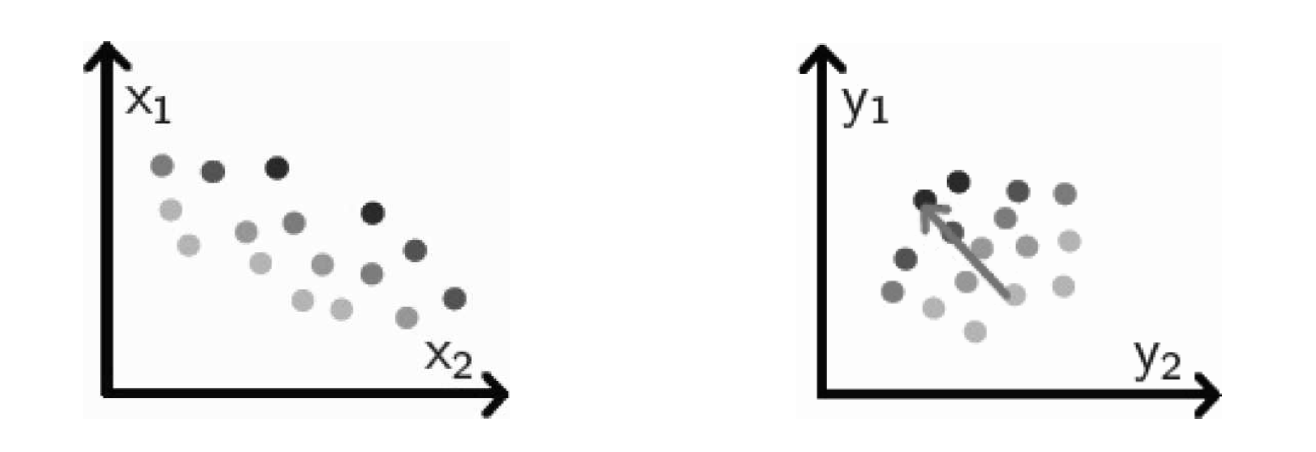
\includegraphics[width=5in]{hw6_template/images/cca.png}
\end{figure}

\item 
\begin{enumerate}[label=(\alph*)]
\item
\begin{lstlisting}[frame=single]
load('data/breast_cancer.mat')

X = X_train ;
Y = Y_train ;
Z = (X.' * X)^(-0.5) * (X.' * Y) * (double(Y.') * double(Y))^(-0.5) ;

[U, S, V] = svd(Z) ; 
corr((X * U(:,1)), (Y * V)) ;
\end{lstlisting}
The correlation is given by $0.9134$. 

\item 
\begin{lstlisting}[frame=single]
[PCAloadings, PCAscores, PCAvar] = pca(X) ;
betaPCR = regress(Y, PCAscores(:,1)) ;
ypred = PCAscores(:,1) * betaPCR ; 

corr(ypred, Y);
\end{lstlisting}
THe correlation between $\hat{y}$ and $y$ is given by $0.9098$. 
\end{enumerate}
\end{enumerate}

\end{homeworkProblem}


\begin{homeworkProblem}

Sensational EM

\solution

\end{homeworkProblem}


\begin{homeworkProblem}

K-Means

\solution

\begin{enumerate}
\item Yes, because 

\item 
\begin{enumerate}[label=(\alph*)]
\item 
\begin{lstlisting}[frame=single]
X = [2 1; 2 2; 3 1; 3 2;
    8 6; 7 7; 7 8; 8 9;
    12 6; 13 7; 13 8; 12 9;
    17 1; 17 2; 17 3];

rng(23) ; 

c_start = [7 7; 8 9; 12 9] ;
[idx1,C1] = kmeans(X, 3, 'MaxIter', 1, 'Start', c_start) ;

figure;
plot(X(idx1==1,1),X(idx1==1,2),'b.','MarkerSize',12);
hold on;
plot(X(idx1==2,1),X(idx1==2,2),'r.','MarkerSize',12);
plot(X(idx1==3,1),X(idx1==3,2),'g.','MarkerSize',12);
plot(c_start(:,1),c_start(:,2),'kx','MarkerSize',15,'LineWidth',3);
text(c_start(1,1)+0.25,c_start(1,2)-0.25,...
['(' num2str(c_start(1,1)) ',' num2str(c_start(1,2)) ')']) ;
text(c_start(2,1)+0.25,c_start(2,2)-0.25,...
['(' num2str(c_start(2,1)) ',' num2str(c_start(2,2)) ')']) ;
text(c_start(3,1)+0.25,c_start(3,2)-0.25,...
['(' num2str(c_start(3,1)) ',' num2str(c_start(3,2)) ')']) ;
legend('Cluster 1','Cluster 2','Cluster 3','Centroids',...
'Location','NorthEast');
hold off;
\end{lstlisting}
Iter 1 plot
\begin{lstlisting}[frame=single]
[idx2,C2] = kmeans(X, 3, 'MaxIter', 1, 'Start', C1) ;

figure;
plot(X(idx2==1,1),X(idx2==1,2),'b.','MarkerSize',12);
hold on;
plot(X(idx2==2,1),X(idx2==2,2),'r.','MarkerSize',12);
plot(X(idx2==3,1),X(idx2==3,2),'g.','MarkerSize',12);
plot(C1(:,1),C1(:,2),'kx','MarkerSize',15,'LineWidth',3);
text(C1(1,1)+0.25,C1(1,2)-0.25,...
['(' num2str(C1(1,1)) ',' num2str(C1(1,2)) ')']) ;
text(C1(2,1)+0.25,C1(2,2)-0.25,...
['(' num2str(C1(2,1)) ',' num2str(C1(2,2)) ')']) ;
text(C1(3,1)+0.25,C1(3,2)-0.25,...
['(' num2str(C1(3,1)) ',' num2str(C1(3,2)) ')']) ;
legend('Cluster 1','Cluster 2','Cluster 3','Centroids',...
'Location','NorthEast');
hold off;
\end{lstlisting}
Iter 2 plot
\begin{lstlisting}[frame=single]
[idx3,C3] = kmeans(X, 3, 'MaxIter', 1, 'Start', C2) ;

figure;
plot(X(idx3==1,1),X(idx3==1,2),'b.','MarkerSize',12);
hold on;
plot(X(idx3==2,1),X(idx3==2,2),'r.','MarkerSize',12);
plot(X(idx3==3,1),X(idx3==3,2),'g.','MarkerSize',12);
plot(C2(:,1),C2(:,2),'kx','MarkerSize',15,'LineWidth',3);
text(C2(1,1)+0.25,C2(1,2)-0.25,...
['(' num2str(C2(1,1)) ',' num2str(C2(1,2)) ')']) ;
text(C2(2,1)+0.25,C2(2,2)-0.25,...
['(' num2str(C2(2,1)) ',' num2str(C2(2,2)) ')']) ;
text(C2(3,1)+0.25,C2(3,2)-0.25,...
['(' num2str(C2(3,1)) ',' num2str(C2(3,2)) ')']) ;
legend('Cluster 1','Cluster 2','Cluster 3','Centroids',...
'Location','NorthEast');
hold off;
\end{lstlisting}
Iter 3 plot
\begin{lstlisting}[frame=single]
[idx4,C4] = kmeans(X, 3, 'MaxIter', 1, 'Start', C3) ;

figure;
plot(X(idx4==1,1),X(idx4==1,2),'b.','MarkerSize',12);
hold on;
plot(X(idx4==2,1),X(idx4==2,2),'r.','MarkerSize',12);
plot(X(idx4==3,1),X(idx4==3,2),'g.','MarkerSize',12);
plot(C3(:,1),C3(:,2),'kx','MarkerSize',15,'LineWidth',3);
text(C3(1,1)+0.25,C3(1,2)-0.25,...
['(' num2str(C3(1,1)) ',' num2str(C3(1,2)) ')']) ;
text(C3(2,1)+0.25,C3(2,2)-0.25,...
['(' num2str(C3(2,1)) ',' num2str(C3(2,2)) ')']) ;
text(C3(3,1)+0.25,C3(3,2)-0.25,...
['(' num2str(C3(3,1)) ',' num2str(C3(3,2)) ')']) ;
legend('Cluster 1','Cluster 2','Cluster 3','Centroids',...
'Location','NorthEast');
hold off;
\end{lstlisting}
Iter 4 plot
\item 
\begin{lstlisting}[frame=single]
c_start = [12 6; 8 9; 12 9] ;
[idx1,C1] = kmeans(X, 3, 'MaxIter', 1, 'Start', c_start) ;

figure;
plot(X(idx1==1,1),X(idx1==1,2),'b.','MarkerSize',12);
hold on;
plot(X(idx1==2,1),X(idx1==2,2),'r.','MarkerSize',12);
plot(X(idx1==3,1),X(idx1==3,2),'g.','MarkerSize',12);
plot(c_start(:,1),c_start(:,2),'kx','MarkerSize',15,'LineWidth',3);
text(c_start(1,1)+0.25,c_start(1,2)-0.25,...
['(' num2str(c_start(1,1)) ',' num2str(c_start(1,2)) ')']) ;
text(c_start(2,1)+0.25,c_start(2,2)-0.25,...
['(' num2str(c_start(2,1)) ',' num2str(c_start(2,2)) ')']) ;
text(c_start(3,1)+0.25,c_start(3,2)-0.25,...
['(' num2str(c_start(3,1)) ',' num2str(c_start(3,2)) ')']) ;
legend('Cluster 1','Cluster 2','Cluster 3','Centroids',...
'Location','NorthEast');
hold off;
\end{lstlisting}
Iter 1 plot
\begin{lstlisting}[frame=single]
[idx2,C2] = kmeans(X, 3, 'MaxIter', 1, 'Start', C1) ;

figure;
plot(X(idx2==1,1),X(idx2==1,2),'b.','MarkerSize',12);
hold on;
plot(X(idx2==2,1),X(idx2==2,2),'r.','MarkerSize',12);
plot(X(idx2==3,1),X(idx2==3,2),'g.','MarkerSize',12);
plot(C1(:,1),C1(:,2),'kx','MarkerSize',15,'LineWidth',3);
text(C1(1,1)+0.25,C1(1,2)-0.25,...
['(' num2str(C1(1,1)) ',' num2str(C1(1,2)) ')']) ;
text(C1(2,1)+0.25,C1(2,2)-0.25,...
['(' num2str(C1(2,1)) ',' num2str(C1(2,2)) ')']) ;
text(C1(3,1)-1.3,C1(3,2)-0.25,...
['(' num2str(C1(3,1)) ',' num2str(C1(3,2)) ')']) ;
legend('Cluster 1','Cluster 2','Cluster 3','Centroids',...
'Location','NorthEast');
hold off;
\end{lstlisting}
Iter 2 plot
\begin{lstlisting}[frame=single]
[idx3,C3] = kmeans(X, 3, 'MaxIter', 1, 'Start', C2) ;

figure;
plot(X(idx3==1,1),X(idx3==1,2),'b.','MarkerSize',12);
hold on;
plot(X(idx3==2,1),X(idx3==2,2),'r.','MarkerSize',12);
plot(X(idx3==3,1),X(idx3==3,2),'g.','MarkerSize',12);
plot(C2(:,1),C2(:,2),'kx','MarkerSize',15,'LineWidth',3);
text(C2(1,1)-1,C2(1,2)-0.25,...
['(' num2str(C2(1,1)) ',' num2str(C2(1,2)) ')']) ;
text(C2(2,1)+0.25,C2(2,2)-0.25,...
['(' num2str(C2(2,1)) ',' num2str(C2(2,2)) ')']) ;
text(C2(3,1)-1.5,C2(3,2)-0.25,...
['(' num2str(C2(3,1)) ',' num2str(C2(3,2)) ')']) ;
legend('Cluster 1','Cluster 2','Cluster 3','Centroids',...
'Location','NorthEast');
hold off;
\end{lstlisting}
Iter 3 plot
\begin{lstlisting}[frame=single]
[idx4,C4] = kmeans(X, 3, 'MaxIter', 1, 'Start', C3) ;

figure;
plot(X(idx4==1,1),X(idx4==1,2),'b.','MarkerSize',12);
hold on;
plot(X(idx4==2,1),X(idx4==2,2),'r.','MarkerSize',12);
plot(X(idx4==3,1),X(idx4==3,2),'g.','MarkerSize',12);
plot(C3(:,1),C3(:,2),'kx','MarkerSize',15,'LineWidth',3);
text(C3(1,1)+0.25,C3(1,2)-0.25,...
['(' num2str(C3(1,1)) ',' num2str(C3(1,2)) ')']) ;
text(C3(2,1)+0.25,C3(2,2)-0.25,...
['(' num2str(C3(2,1)) ',' num2str(C3(2,2)) ')']) ;
text(C3(3,1)-1,C3(3,2)-0.25,...
['(' num2str(C3(3,1)) ',' num2str(C3(3,2)) ')']) ;
legend('Cluster 1','Cluster 2','Cluster 3','Centroids',...
'Location','NorthEast');
hold off;
\end{lstlisting}
Iter 4 plot
\begin{lstlisting}[frame=single]
[idx5,C5] = kmeans(X, 3, 'MaxIter', 1, 'Start', C4) ;

figure;
plot(X(idx5==1,1),X(idx5==1,2),'b.','MarkerSize',12);
hold on;
plot(X(idx5==2,1),X(idx5==2,2),'r.','MarkerSize',12);
plot(X(idx5==3,1),X(idx5==3,2),'g.','MarkerSize',12);
plot(C4(:,1),C4(:,2),'kx','MarkerSize',15,'LineWidth',3);
text(C4(1,1)+0.25,C4(1,2)-0.25,...
['(' num2str(C4(1,1)) ',' num2str(C4(1,2)) ')']) ;
text(C4(2,1)+0.25,C4(2,2)-0.25,...
['(' num2str(C4(2,1)) ',' num2str(C4(2,2)) ')']) ;
text(C4(3,1)-1,C4(3,2)-0.25,...
['(' num2str(C4(3,1)) ',' num2str(C4(3,2)) ')']) ;
legend('Cluster 1','Cluster 2','Cluster 3','Centroids',...
'Location','NorthEast');
hold off;
\end{lstlisting}
Iter 5 plot
\end{enumerate}
\end{enumerate}
\end{homeworkProblem}


\begin{homeworkProblem}

Principal Components Analysis

\solution

\begin{enumerate}
\item 
\begin{lstlisting}[frame=single]
load('data/MNIST_train.mat') ;
load('data/MNIST_test.mat') ;

rng(147) ;

[PCAloadings, PCAscores, PCAvar, tsquared, explained] = pca(X_train) ;

proj1 = PCAscores(Y_train==1,:);
proj2 = PCAscores(Y_train==2,:);

figure;
plot(proj1(:,1),proj2(:,1),'ob','MarkerSize',6);
hold on;
plot(proj1(:,2),proj2(:,2),'+m','MarkerSize',6);
xlabel('PC1') ;
ylabel('PC2') ;
title('Test digits for the first 2 PCA dimensions') ;
legend('PCA 1','PCA 2','Location','NorthEast');
hold off;
\end{lstlisting}
plot

\item 
\begin{lstlisting}[frame=single]
mu = mean(X_train) ;
nPC = size(PCAloadings, 2);

err_mat = zeros(nPC, 2);
err_mat(:,1) = 1:nPC;

for pcnum = 1:nPC 
  xhat = PCAscores(:,1:pcnum) * PCAloadings(:,1:pcnum)' ;
  xhat = bsxfun(@plus, xhat, mu) ;

  reconstruct_err = sqrt(sum(bsxfun(@minus, X_train, xhat).^2, 2)) ;
  
  err_mat(pcnum, 2) = mean(reconstruct_err) ;

end

figure;
plot(1:nPC, err_mat(:,2));
xlabel('Principal Components included') ;
ylabel('Average reconstruction error') ;
title({'Average reconstruction error as a function','of principal components included'}) ;
\end{lstlisting}
plot
\begin{lstlisting}[frame=single]
PCvariation = cumsum(explained) ;
minPC = find(PCvariation >= 85, 1) ;
\end{lstlisting}
The number of principal components needed to explain $85\%$ of the variation is.

\item For a 100 dimensions,
\begin{lstlisting}[frame=single]
numdim = 100 ;
[idx, C] = kmeans(PCAscores(:,1:numdim), 10) ;

test_center = bsxfun(@minus, X_test, mean(X_test)) ; 
project_test = test_center * PCAloadings(:,1:numdim) ;
precision = k_means(PCAscores(:,1:numdim), Y_train, project_test, Y_test, 10);
\end{lstlisting}
giving an accuracy of .\\
For 150 dimensions, 
\begin{lstlisting}[frame=single]
numdim = 150 ;
[idx, C] = kmeans(PCAscores(:,1:numdim), 10) ;

test_center = bsxfun(@minus, X_test, mean(X_test)) ; 
project_test = test_center * PCAloadings(:,1:numdim) ;
precision = k_means(PCAscores(:,1:numdim), Y_train, project_test, Y_test, 10);
\end{lstlisting}
giving an accuracy of .\\
For 200 dimensions,
\begin{lstlisting}[frame=single]
numdim = 200 ;
[idx, C] = kmeans(PCAscores(:,1:numdim), 10) ;

test_center = bsxfun(@minus, X_test, mean(X_test)) ; 
project_test = test_center * PCAloadings(:,1:numdim) ;
precision = k_means(PCAscores(:,1:numdim), Y_train, project_test, Y_test, 10);
\end{lstlisting}
giving an accuracy of.

\item blah

\item We run the exact same code as in part 3 with all instances of 10 replaced by 25. For 100 dimensions,
\end{enumerate}
\end{homeworkProblem}

\end{document}


